\chapter{Our Approach}
\label{sec:our-approach}

We propose and discuss a system architecture for a backup system in the first section of this chapter and explain the underlying design decisions in the second section. The third section presents the structure and testing results of a prototype, which implements a subset of the proposed system.

We illustrate architecture structure using the C4 model for software architecture\footnote{\url{https://c4model.com/}}.

\section{System Architecture}
% Brief introdcution of all actors, components and messages
% The specification is complicated because it is the result of long discussions and a clarification process (see https://project.redbackup.org/browse/REDPRO-98)
% See Describing architectures in https://wiki.hsr.ch/FarhadMehta/files/Writing_Scientific_Papers.pdf
% Describe everything concise and with exact definitions.
% Use schemes and flowcharts

\paragraph{Actors} There are two kinds of actors interacting with the system. A typical \gls{user} wants to store backups in the redbackup system and restore them (partially) when needed. The other kind of actor is an \gls{administrator} that configures the system, e.g. extends storage capacity or replaces corrupted disks.

\begin{figure}[h]
	\centering
	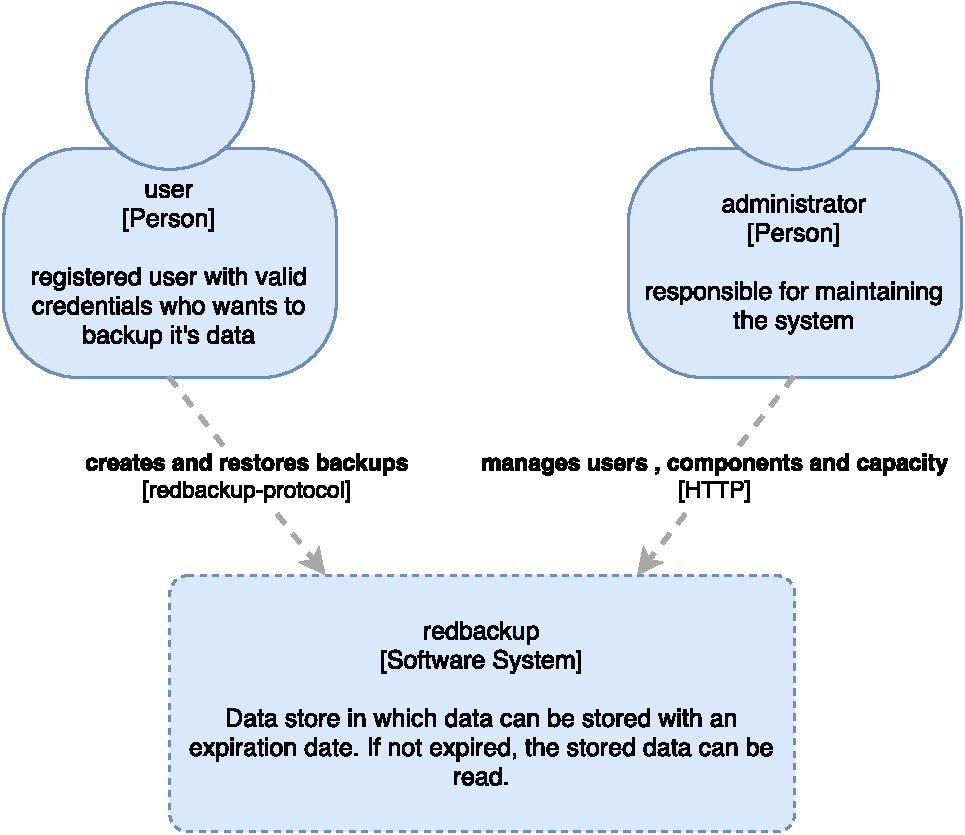
\includegraphics[width=0.8\linewidth]{resources/c4-overview}
	\caption[C4 System Context diagram]{C4 System Context diagram showing the big picture.}
	\label{fig:c4-overview}
\end{figure}

Distinctive for both actors is that they do not want to interact directly with the system unless human interaction is inevitable. This takes the burden to manually create backups from the user including the risk of oblivion and minimises \gls{management} efforts required by the administrator.  

Both actors, as well as their intentions, are described in more detail in Appendix \fullref{sec:specification}. Figure \ref{fig:c4-overview} presents a high-level overview that illustrates the interactions of the actors with the redbackup system.

\paragraph{Structure}
The redbackup system consists of four core components as shown in the C4 Container diagram in Figure \ref{fig:c4-container}.

\begin{figure}[h]
	\centering
	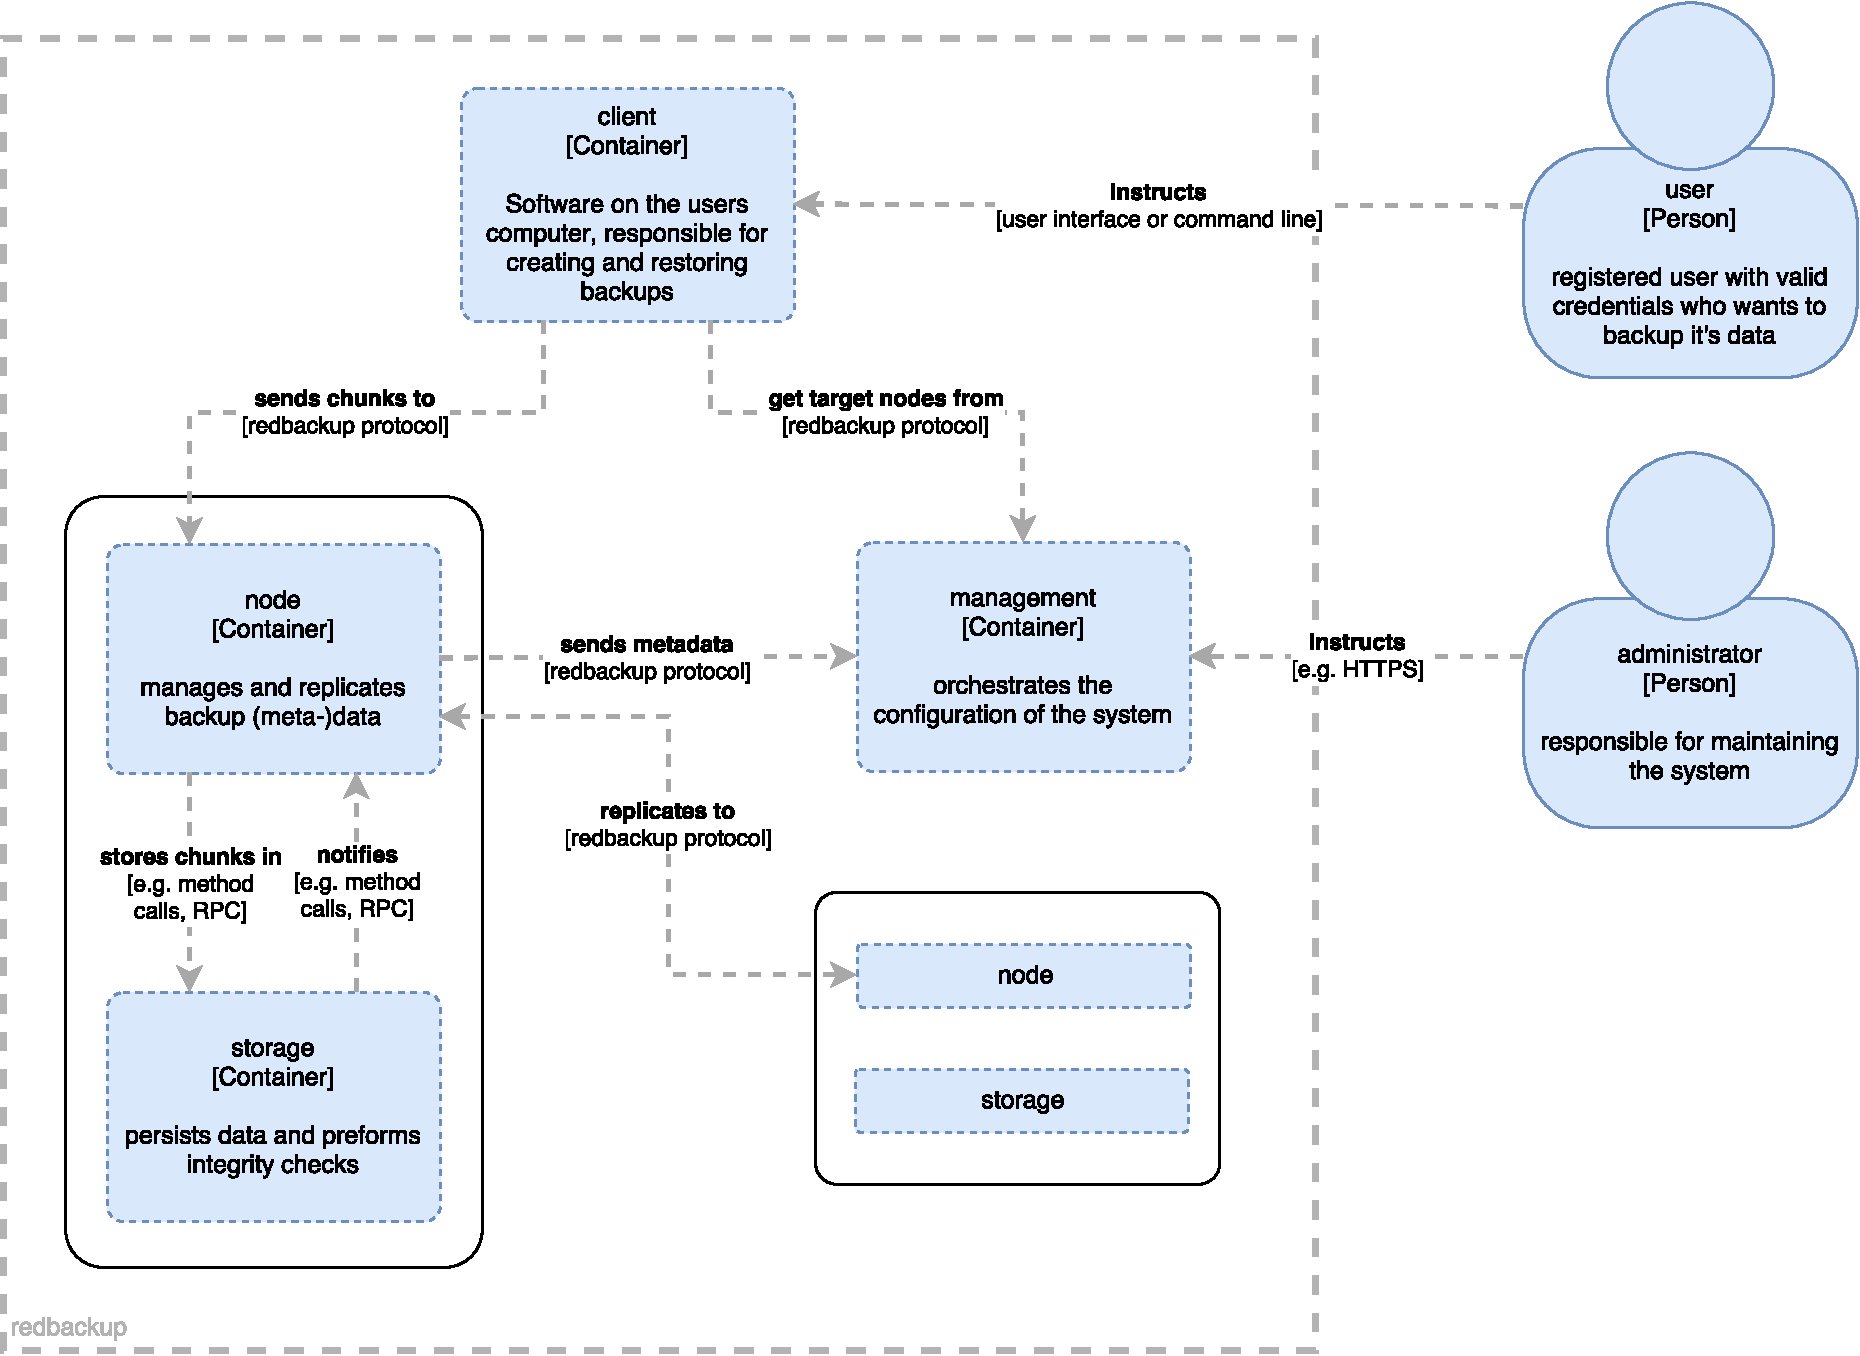
\includegraphics[width=1\linewidth]{resources/c4-container}
	\caption[C4 Container diagram]{C4 Container diagram illustrating the high-level shape of the redbackup software system and how responsibilities are distributed.}
	\label{fig:c4-container}
\end{figure}

\paragraph{Client} A \gls{user} instructs a \gls{client} program typically running on the users machine to perform (unattended) backups and restores.  A \gls{client} persists and loads its data from one or more interconnected \glspl{node}.

\paragraph{Node}
A \gls{node} then is in charge of the data \glspl{chunk} including their replication onto other \glspl{node}. \Glspl{node} persist the actual data in a separate component, a \gls{storage}, to encapsulate persistence from replication and interaction to support different kinds of storage technologies (e.g. plain file systems or databases). A \gls{node} and its \gls{storage} are typically deployed on the same host.

\paragraph{Management}
One central \gls{management} component orchestrates the configuration of the system by providing metadata to \glspl{client} and \glspl{node}. This metadata includes user information and a set of all \glspl{node} in the system including their addresses and states. Clients and \glspl{node} must cache this metadata which ensures that a temporary unavailability of the \gls{management} component does not compromise the replication and backup process.

All components including their responsibilities and interactions are described in more detail in Appendix \fullref{sec:specification}.

\paragraph{Protocols} Redbackup specifies a high-level protocol that is used for internal communication (noted in all C4 diagrams as \emph{redbackup protocol}). We deliberately specified the communication on a high level to encapsulate the underlying protocol.

In the prototype, we used a custom, minimal protocol that is based on TCP and sends framed Message Pack\footnote{\url{https://msgpack.org/}} encoded messages. If we decided to switch to e.g. HTTP as the underlying protocol to overcome firewall issues in the future, only these forwarder and receiver components have to be adapted while the actual message format does not change. 

\subsection{Backup creation}
\begin{figure}[h]
    \centering
    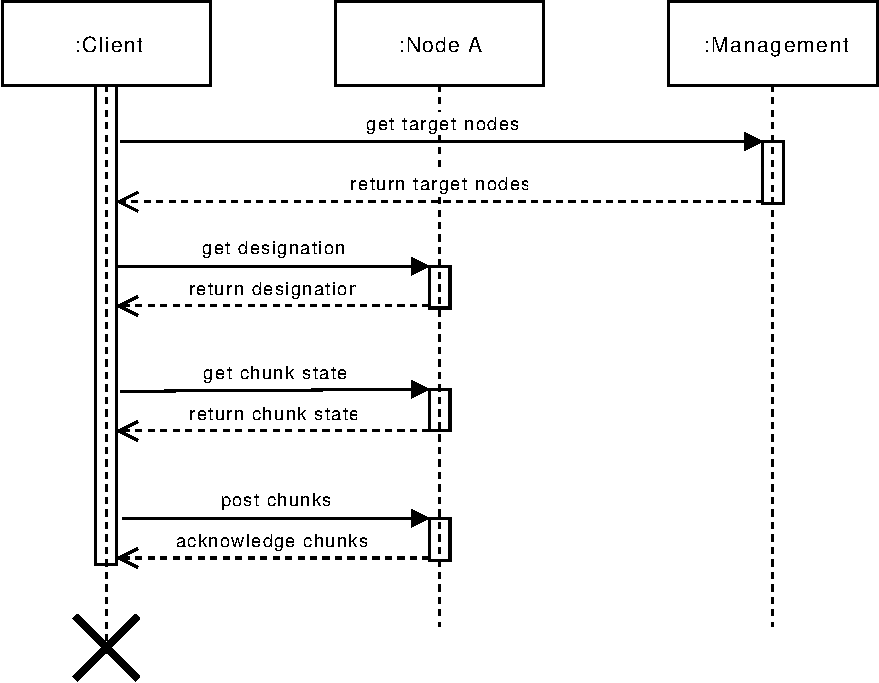
\includegraphics[width=\linewidth]{resources/create_backup}
    \caption{Create Backup UML Sequence Diagram}
\end{figure}

To create a backup, a \gls{client} loads a set of \glspl{node} including their addresses from the \gls{management}. The \gls{client} caches this set and chooses one of them as \gls{designated-node}. This selection can either be random or based on heuristics, e.g. by analysing the round trip time to the \gls{node}.

The \gls{client} then requests permission to perform a backup on a given \gls{designated-node} by sending a \emph{get designation} message that includes an estimated backup size and the \gls{expiration-date}. If the \gls{designated-node} has the storage capacity as well as other resources available (i.e. it is not under overload), it confirms the designation request.

By now, the \gls{client} must start to build up backup metadata - hereafter called \gls{chunk-index} - by walking recursively through all directories to back up. Each file that is not explicitly excluded is split up into one or more data \glspl{chunk} using a rolling hash\cite{borg-data-structures}. Each of these \glspl{chunk} are then encrypted individually. Afterwards the \gls{client} derives the identifier of every \gls{chunk} based on its contents. This mechanism enables deduplication. Section \fullref{sec:fundamental-design-decisions} discusses \glspl{chunk} and \glspl{chunk-identifier} detail.

The \gls{client} sends the calculated \glspl{chunk-identifier} at regular intervals to the \gls{designated-node}. The \gls{designated-node} returns a subset of all \glspl{chunk-identifier} of the \glspl{chunk} that are already present on it.

The \gls{client} then posts the missing data \glspl{chunk} to the \gls{designated-node} which acknowledges after successful receipt.

When all \glspl{chunk} are transmitted successful, the client encrypts the backup metadata as well and sends to the \gls{designated-node} using the same mechanism as for any other \gls{chunk}. The only difference is that an additional flag - hereafter called \gls{root-handle} - is set so that it can be found again for restore.

The detailed scenario description including all edge cases are described in Appendix \fullref{sec:scenario-create-backup}.

\subsection{Backup restore}

\begin{figure}[h]
    \centering
    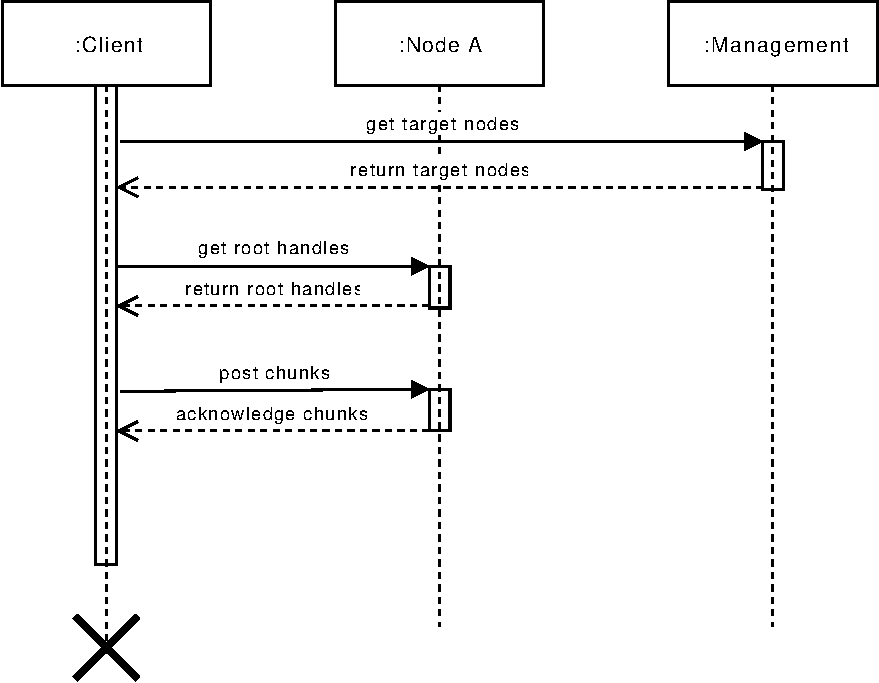
\includegraphics[width=\linewidth]{resources/backup_restore.pdf}
    \caption{Backup Restore UML Sequence Diagram}
\end{figure}

The restore mechanism starts identically to the backup process until a \gls{designated-node} is chosen.

Next, the \glspl{client} loads all \glspl{root-handle} from the \gls{designated-node}. The \glspl{client} can decrypt the backup metadata, the \gls{chunk-table}, from the returned \glspl{chunk-content}. Based on this information, the \gls{client} can provide multiple restore options to the \gls{user}, e.g. to restore a particular version of a given file.
Based on the user input and the previously fetched \glspl{chunk-table}, the \glspl{client} can calculate which \glspl{chunk} must be requested from the \gls{designated-node}. These \glspl{chunk-content} are then loaded at regular intervals from the \gls{designated-node}, decrypted and combined.

\subsection{Replication}
% Planned and unplanned leaving of nodes
% Management down

We deliberately specified \emph{n-replication} only, which means the degree of redundancy for the whole system is equal to the amount of \glspl{node} in the system (see \fullref{sec:fundamental-design-decisions}).

A \gls{node} is in charge for all data stored on it. Each \gls{node} - hereafter called \gls{sending-node} - randomly picks $n$ of its data \glspl{chunk}. It then picks one other \gls{node} randomly - hereafter called \gls{designated-node} - and requests which of the chosen data \glspl{chunk} are persisted on the \gls{designated-node}. The \gls{designated-node} returns a subset of the requested \glspl{chunk} that consists of all \glspl{chunk} that it owns. Using this response, the \gls{sending-node} sends all missing \glspl{chunk} to the \gls{designated-node} which acknowledges after successful receipt.

\begin{figure}[h]
    \centering
    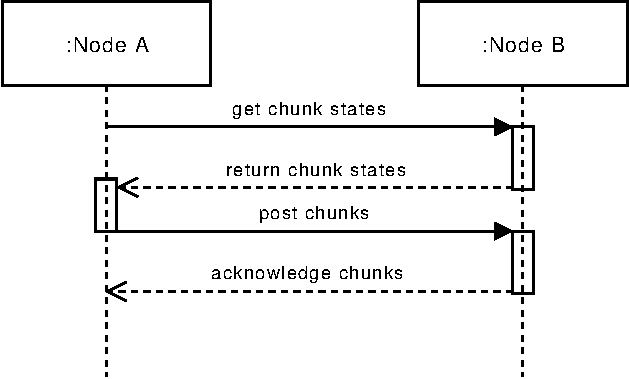
\includegraphics[width=0.6\linewidth]{resources/data_replication.pdf}
    \caption{Data Replication UML Sequence Diagram}
\end{figure}

This scenario is described in more detail in the Appendix \fullref{sec:scenario-data-replication}.

\subsection{Security and Encryption}\label{sec:security-and-encryption}
\paragraph{Data Integrity} One of our primary design goals is to ensure that once data is in the redbackup system, it can not be altered or deleted from a \gls{client} to prevent ransomware attacks \cite{young-cryptovirology}. To achieve this, each backup is created with an \gls{expiration-date} on which \glspl{node} are allowed to remove the associated data. 

Reasoning and potential risks of physical time are discussed in paragraph \fullref{sec:removal-of-old-backups}.

\paragraph{Data Integrity on Nodes} Because \glspl{node} can also be the target of randsomware attacks, each \gls{node}, or more precisely its associated \gls{storage} component, must verify that given data \gls{chunk} contents are not corrupted using cryptographic hash functions, also known as checksums. To be able to do so, it must be possible to calculate the identifier of such a data \gls{chunk} from its contents.

A discussion on the role of hash functions including the chosen algorithms for the study project is carried out in section \fullref{sec:hash-collisions}.

\paragraph{Data Integrity on the Management} The \gls{management} component has no knowledge of the persisted data in the system and has only knowledge of the configuration (need-to-know principle \cite{security-patterns}).

\paragraph{Data Encryption} A \gls{client} encrypts backup data \glspl{chunk} when creating a new backup. This ensures that no other participant in the redbackup system can inspect file contents (need-to-know principle \cite{security-patterns}). The encryption and decryption keys are only persisted on the \gls{client} and must be backed up separately.

\paragraph{Transport Security} All sent \glspl{message} should be signed by the sender. If so, transport layer encryption is not strictly necessary because all user data is already encrypted on the \gls{client} with the only exception of the \gls{expiration-date}.

A detailed description of these security mechanisms is out of scope for this study project and has to be carried out in the future.

\subsection{Partitioning \& Scaling}

\paragraph{Availability \& Overload} To scale the redbackup system regarding availability and safety, more \glspl{node} can be added to the redbackup system. If a given \gls{node} is overloaded, a \gls{client} can use another \gls{node} for its backup creation or restore.

Because both processes require approval of a chosen \gls{node} (see scenarios \fullref{sec:scenario-create-backup} and \fullref{sec:scenario-backup-restore}), an overloaded \gls{node} can finish work in progress backups/restores and reject new requests (following the patterns Finish Work In Progress and Shed Load \cite{fault-tolerance}). The data is replicated to the overloaded \glspl{node} eventually.

We ensured that \glspl{node} are (mostly) stateles which simplifies scaling as well.

\paragraph{Storage Scalability} Because the proposed system does currently only support \emph{n-replication} (see section \fullref{sec:fundamental-design-decisions}), the maximum storage capacity is the lowest storage size of any \gls{node}. Therefore, to increase storage capacity, the capacity of all \glspl{node} must be extended to the desired amount.

To minimise network usage deduplication of data is used on the \gls{client}. Deduplication is  discussed in the paragraph Storage Unit in  \fullref{sec:fundamental-design-decisions}.

\subsection{Failure Detection}

Additionally to the above-discussed mechanisms for fault tolerance regarding security and scaling, the following failure detection mechanisms are in place.

\paragraph{Reporting} Most issues that occur on a \gls{node} are reported to the \gls{management} component (following the pattern Someone in Charge \cite{fault-tolerance}). The \gls{management} can then decide to notify the system administrator or execute error mitigation processes, e.g. suspend a given \gls{node} temporarily.

If a \gls{node} tries to connect to another \gls{node} that is not available, it notifies the \gls{management} component (following the pattern System Monitor\cite{fault-tolerance}).

Each \gls{node} periodically verifies the persisted contents for possible corruption using the checksum mechanisms discussed in \fullref{sec:security-and-encryption} (following the Pattern Routine Audits \cite{fault-tolerance}). If a corruption is detected, the \gls{storage} notifies the \gls{node} which notifies the \gls{management}.

\paragraph{Single Point of Failure} In case the \gls{management} component is temporarily unavailable, \glspl{node} and \glspl{client} cache configuration data, e.g. information about other \glspl{node}. Using this caches, \glspl{node} can perform replication and \glspl{client} manage their backups without interruption. Any notifications that were not successfully transmitted to the \gls{management} must be buffered on the \glspl{node} as well to ensure their delivery.

\section{Fundamental Design Decisions}\label{sec:fundamental-design-decisions}

We used the morphological box technique to explore different possible solutions (see Table \ref{tbl:morphological-box}). The chosen option should be as simple as possible for the prototype developed in the study project but extensible for further adaption.

The following paragraphs reason the selected entry in each dimension.

\paragraph{Redundancy}
We originally planned to support \emph{client m-replication}, which means that the \gls{client} defines a custom degree of redundancy from 1 to the number of \glspl{node} in the system. However, this is a complex mechanism that requires sophisticated algorithms to work correctly and efficiently. For the prototype, we chose the more straightforward to implement option system \emph{n-replication}, where the degree of redundancy for the whole system is equal to the number of \glspl{node} in it. Changing this option in the future is hard because it requires fundamental changes in the replication process and the communication protocols.

\paragraph{Storage Unit}
The idea of \emph{chunks} come from Borg Backup. Files are partitioned into chunks using a rolling hash which enables deduplication and space efficient backups for large files \cite{borg-data-structures}. These are desired properties in a backup system to minimise network and disk usage.

\emph{Encrypting chunks} means that deduplication of the same file coming from different users is not possible anymore but is a necessity for privacy. Encryption is not trivial and requires a user concept that is out of scope of the prototype developed in the study project.
We chose the \emph{plain files} option for the study project to simplify the \gls{client} implementation. Supporting \emph{encrypted chunks} in the future is possible by just modifying the \gls{client}.

\paragraph{Role of the Management}
The \emph{one in charge} option is the most straightforward option to implement, but conflicts with many intentions of the administrator (see \fullref{sec:adminstrator-intention}). We also intended to avoid a single point of failure. We chose the option \emph{autonomous replication} because it guarantees that replication is always ensured and keeps communication relatively simple.

\paragraph{Storage Backend}
Using the file system is the simplest possible solution for the study project and therefore selected option. Adding support for other backends in the future is still possible since the storage component is an isolated part of the architecture (see \fullref{sec:component-storage}).

The number of files in a folder is limited depending on the used file system, length of a filename and other factors. Some file systems (e.g. ext4) have a global limit for the maximal number of files. This limit is 4 billion files for ext4. \cite{ext4}. Therefore we use the ext4 file system to persist data in the study project.

\paragraph{Removal of Old Backups}\label{sec:removal-of-old-backups}
We propose to use a fixed \emph{physical time} that must be specified on backup creation. After expiration, the backup data may be removed by a garbage collector. This may be extended to allow only mutual garbage removal in the future.

A significant problem that \emph{physical time} addresses is the safety of backup data in case a user computer is infected with malware. An illicit application might command the removal of backups, or create new backups to initiate a garbage collection process to free storage capacity.

Nevertheless, the use of \emph{physical time} has the downside of possible data loss due to wrong system times. To mitigate this risk, the system should use multiple distinct upstream time-servers. This is given with a high probability, as the proposed redundancy model motivates users to expand the system across multiple physical locations. Furthermore, the client, \glspl{node} and \gls{management} should verify a reasonable accurate time when communicating mutually.

\paragraph{Programming Language / Ecosystem}
A complete language evaluation can be found in \fullref{sec:language-evaluation}.

\begin{sidewaystable}
	\centering
	\caption[Morphological Box]{Morphological Box}
	\label{tbl:morphological-box}
    \begin{tabu}{X | X X X X}
		\hline
          \textbf{Redundancy}
          & No redundancy
          & Client m-replication: The \gls{client} defines a custom degree of redundancy (from 1 to the number of \glspl{node}).
          & System m-replication: The administrator defines the degree of redundancy for the whole system (from 1 to the number of \glspl{node}).
          & \textbf{System n-replication}: The degree of redundancy for the whole system is equal to the amount of \glspl{node} in the system.
          \\ \hline

          \textbf{Storage unit}
          & \textbf{Plain files}
          & Encrypted files
          & Chunks: Cut files into multiple parts and store these individually.
          & Encrypted chunks: Same as chunks, but every chunk is individually encrypted.
          \\ \hline


          \textbf{Role of the management}
          & One in charge: The management knows and controls everything (e.g. the location of every file/chunk).
          & Configuration only: The management must be up for administrative tasks only. The \glspl{node} are mostly autonomous.
          & \textbf{Autonomous replication}: The management must be available for most of the tasks but replication also works if the management is down.
          & No management: Every \gls{node} is completely autonomous.
          \\ \hline


          \textbf{Storage backend}
          & \textbf{Plain filesystem}: Store all files/chunks as files in one directory with a unique identifier.
          & Database: Use an existing database solution (e.g. Git, Redis, RocksDB).
          & Cloud Storage: A proxy to a cloud storage provider (e.g. Amazon S3).
          & Custom: An optimized version of the plain file system option with optimised indexing and compression.
          \\ \hline


          \textbf{Removal of old backups}
          & \textbf{Physical time}: Data is removed on a specified physical time.
          & User command: The user commands removal of data.
          & Free storage: Data is removed, as soon as capacity issues occur.
          & Physical time with mutual agreement: All \glspl{node} must agree before data is removed.
          \\ \hline


          \textbf{Programming language / ecosystem}
          & \textbf{Rust}
          & Go
          & Erlang
          & 
          \\ \hline
	\end{tabu}
\end{sidewaystable}

\subsection{Hash Collisions}\label{sec:hash-collisions}
To achieve deduplication and space-efficient backups for large files, as discussed above, a file/chunk identifier must be derived from the actual file/chunk contents. 
A common mechanism used to derive identifiers from binary data is the use of cryptographic hash functions. Most cryptographic hash functions produce a message digest having a fixed size (e.g. SHA-256\cite{sha-256} produces a 256-bit digest) for a message with an arbitrary length, which can theoretically lead to collisions.
Perfect hash functions do not have this property because their input message size is fixed and equal to the size of the resulting message digest. A perfect hash function is not practical in our case due to the large message digests.
With cryptographic hash functions, collisions are possible but unlikely. Assuming that the applied function does produce equally distributed results, the probability can be calculated based on the birthday problem\cite{birthday-attack} as follows, where $p$ is the number of chunks in the system and $n$ the size of the message digests:

\[
P(p, n) = \frac{p^2}{2^{n+1}}
\]

Assuming we have $p=30^{21}$ files/chunks the system (which is equivalent to two billion years of music assuming each chunk has a size of one byte\cite{seagate-zetabyte}) and using the SHA-256 algorithm, the probability of collisions is about $4.72 \cdot 10^{-16}$, which is highly improbable and may therefore be neglected.

However, if a collision would happen after all, for example, if the used cryptographic hash function is flawed or the unlikely event occurs, it results in data loss.

In theory, we could detect collisions on the \gls{client}. To do so, every time an identifier is calculated, the \gls{client} must verify that if a file with the same identifier exists already in the system, it has the exact same contents. If the contents differ, it is a collision. This approach requires a lot of network traffic and can slow down the backup process significantly.

Another place to detect collisions is on the \gls{node}. A \gls{node} can verify if the contents of a given file/chunk are equal to the contents already present in the system. The downside of this approach is that it requires the \gls{client} always to send the full contents of every file, which means there is a lot of additional network traffic.

Both of the described approaches for collision detection have significant costs that are not practical.

As for the study project, we use the SHA-256 algorithm\cite{sha-256} and neglect the risk of hash collisions due to its low probability. Nonetheless, we prepare all protocols and components to use an interchangeable mechanism for the calculation and transmission of file/chunk identifiers.

\section{Prototype}

Because the whole system as described in the previous sections is too large and complex to implement in the form of a study project prototype, we reduced the functionality to its core.

Our prototype focuses on the backup, restore and replication scenarios as described in Appendix \fullref{sec:scenarios} leaving out encryption.

We also limited the supported plattforms to 64-Linux only as this is the operating system we use for development and continous integration.

\subsection{Concrete Architecture}

Figure \ref{fig:c4-sa-container} illustrates the system as implemented in our prototype.

The \gls{client} and \gls{node} are delivered as executables that are be configured and launched using the command line.

The \gls{node} component binds itself to a provided network interface and port on which it provides the services for backup creation, backup restore and replication.

The \gls{client} binary is started individually for every operation, that is the creation of a backup, listing all backups persisted on a given \gls{node} and data restore.

All components are implemented using the Rust programming language \cite{rustlang-org}. Installation instructions are documented in the project's repository.

\begin{figure}[h]
	\centering
	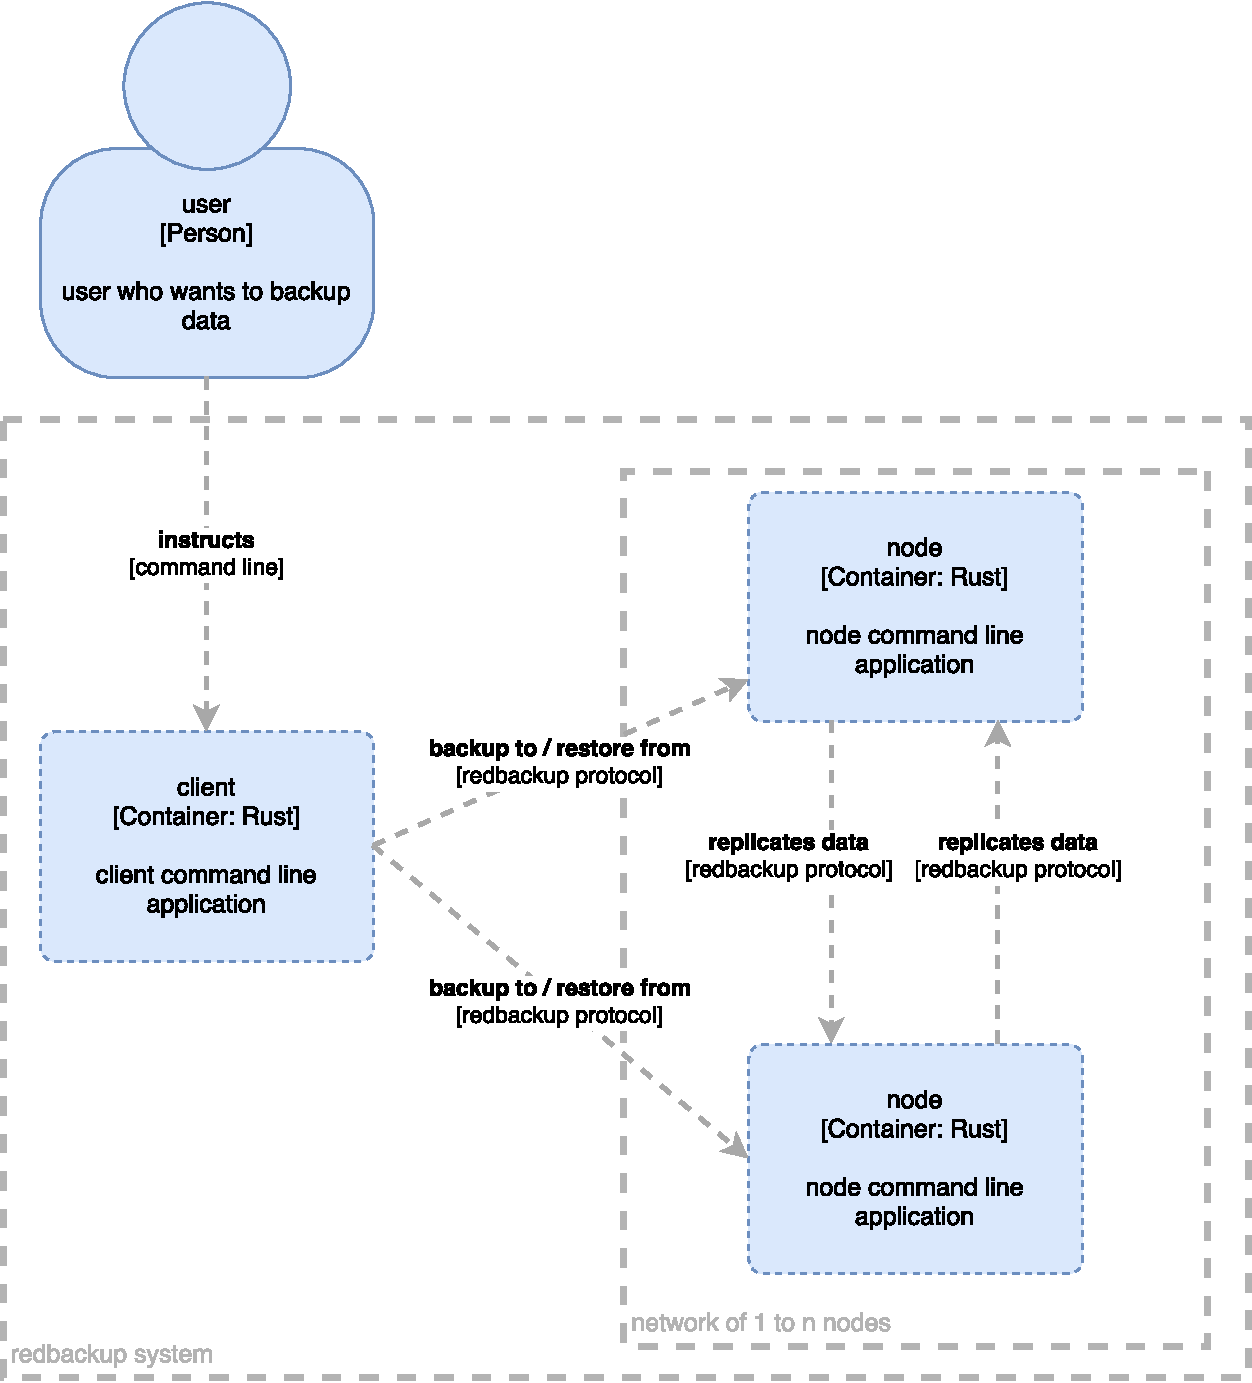
\includegraphics[width=1\linewidth]{resources/c4-sa-container}
	\caption[SA specific C4 Container diagram]{C4 Container diagram illustrating the high-level shape of the prototype and how responsibilities are distributed as implemented in the study project.}
	\label{fig:c4-sa-container}
\end{figure}

\subsubsection{Client}

The \gls{client} executable bundles three components as shown in Figure \ref{fig:c4-client-container}.

\begin{figure}[h]
	\centering
	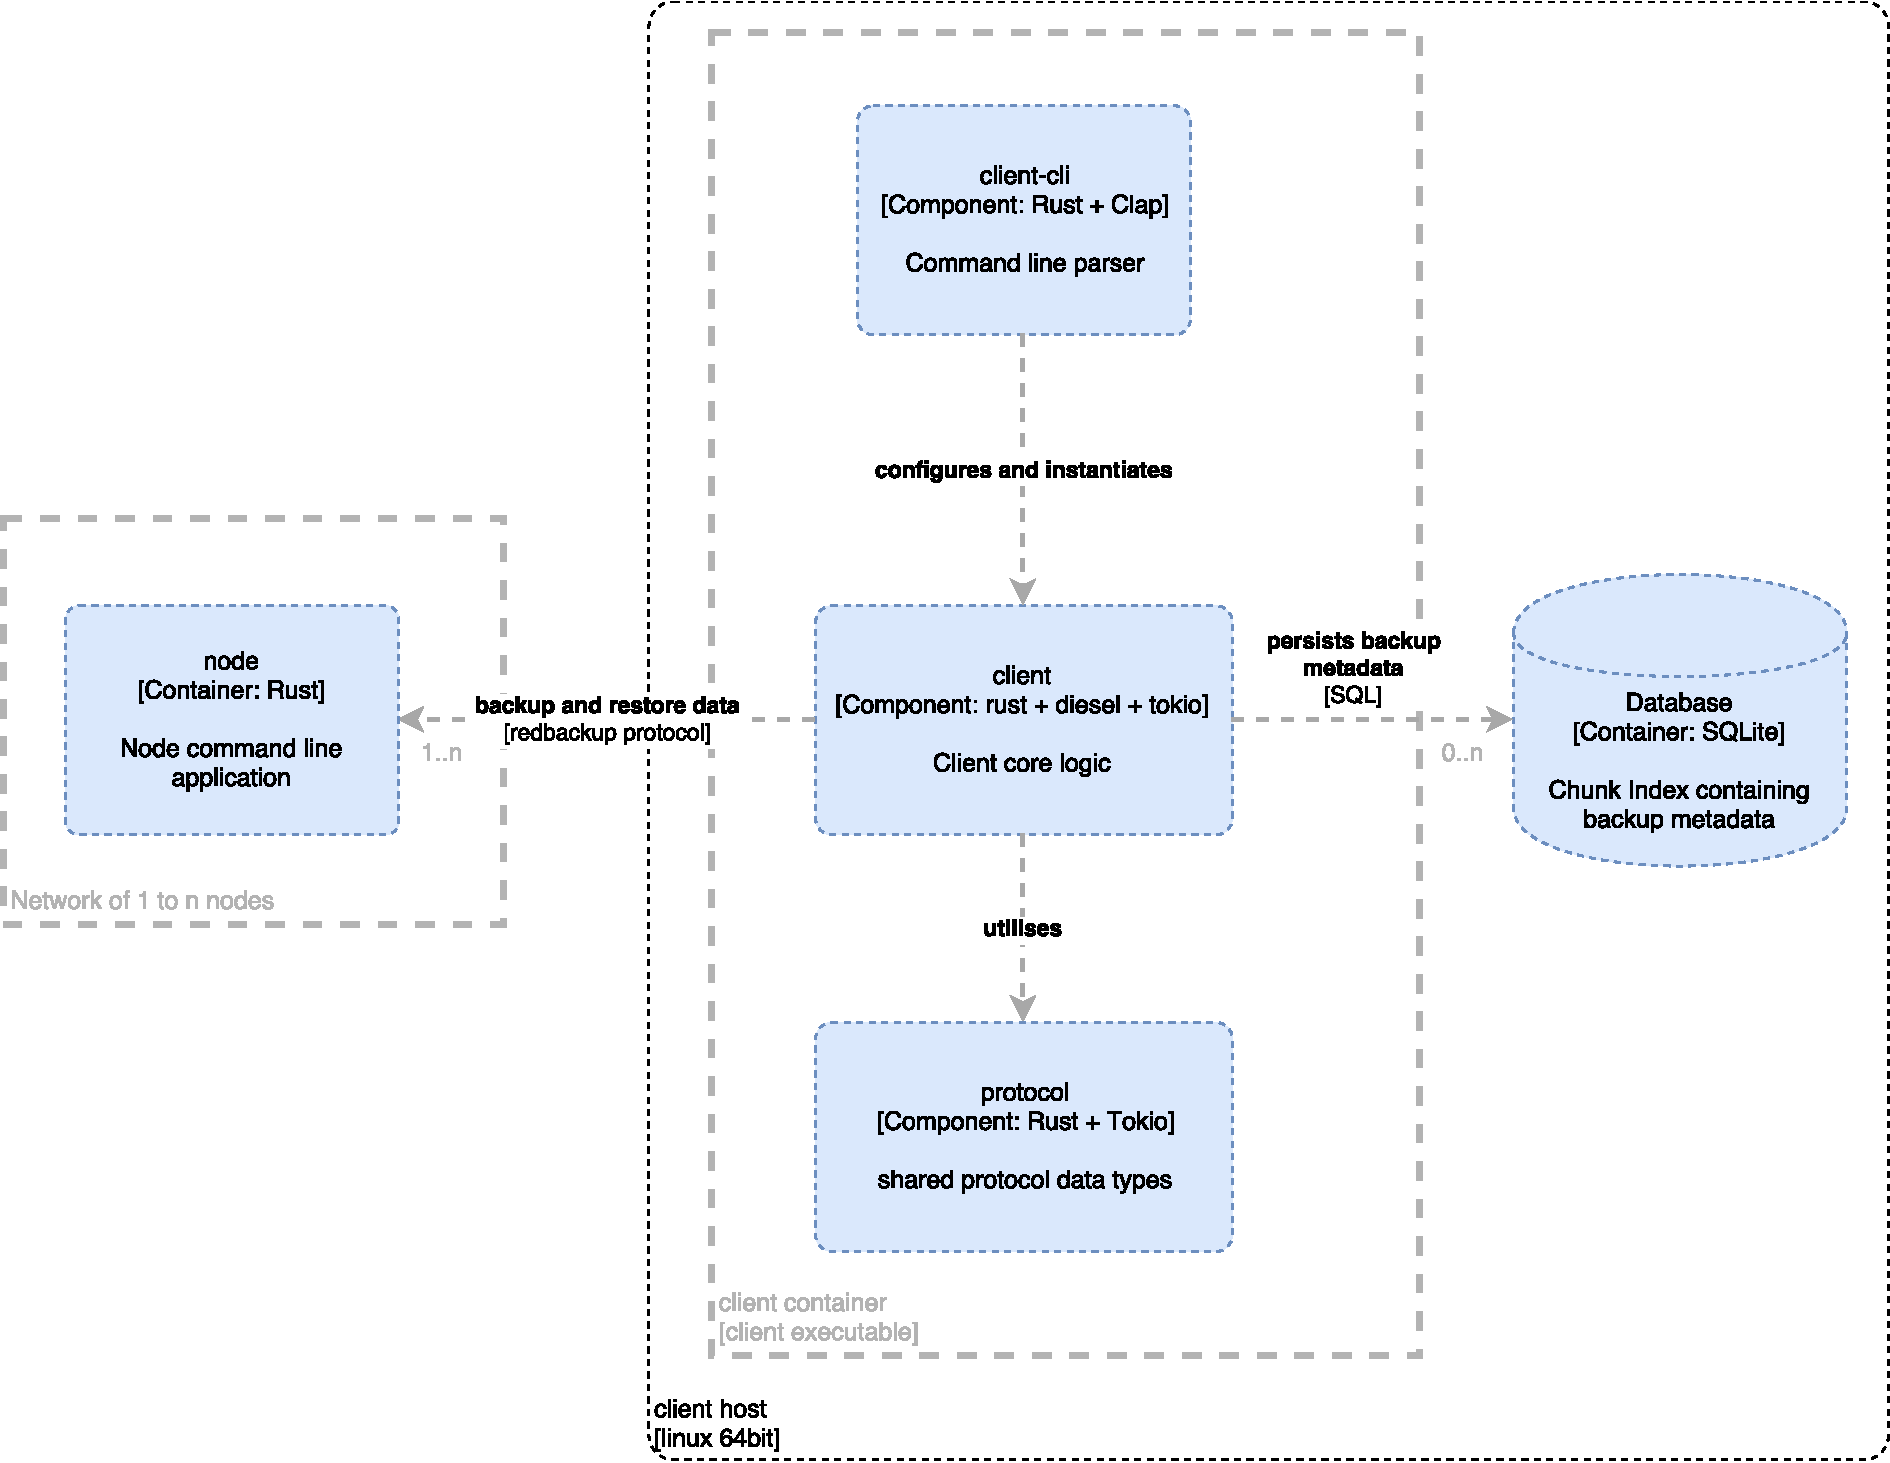
\includegraphics[width=1\linewidth]{resources/c4-client-container}
	\caption[Client specific C4 Container diagram]{C4 Container diagram illustrating the shape of the \gls{client} and how responsibilities are distributed as implemented in the study project.}
	\label{fig:c4-client-container}
\end{figure}

\emph{Client-cli} contains the command line specific logic that provides an uncluttered interface for advanced users and serves as an entry point in the client's core logic. We used the clap\footnote{\url{https://clap.rs/}}  library to implement this component.

The \emph{client} component contains the actual logic for creating and restoring backups. It is organised as a library so that it can be used for other projects as well, e.g. if we provide a graphical user interface in the future. The \gls{client} component creates metadata for every backup in a separate \emph{SQlite-database}. These databases are also the entry point for a restore. For database access, we used the Diesel\footnote{\url{https://diesel.rs/}} ORM-library.

The \gls{client} components make heavy use of a networking library called tokio\footnote{\url{https://tokio.rs/}} that provides an efficient event loop similar to the Reactor pattern \cite{POSA1}. Although tokio supports highly parallel networking code, we decided to implement all interactions from a \gls{client} to \glspl{node} serial to keep it simple and readable.

The (de-) serialisation mechanisms for messages sent to \glspl{node} are encapsulated in the \emph{protocol} component (Forwarder Receiver Pattern \cite{POSA1}).

In this prototype, the \gls{client} interacts with one \gls{node} at a time to maintain simplicity. The \gls{node} to interact with is passed to the \gls{client} executable via command line arguments.

\subsubsection{Node}

The \gls{node} executable bundles four components as shown in Figure \ref{fig:c4-node-container}.  

\begin{figure}[h]
	\centering
	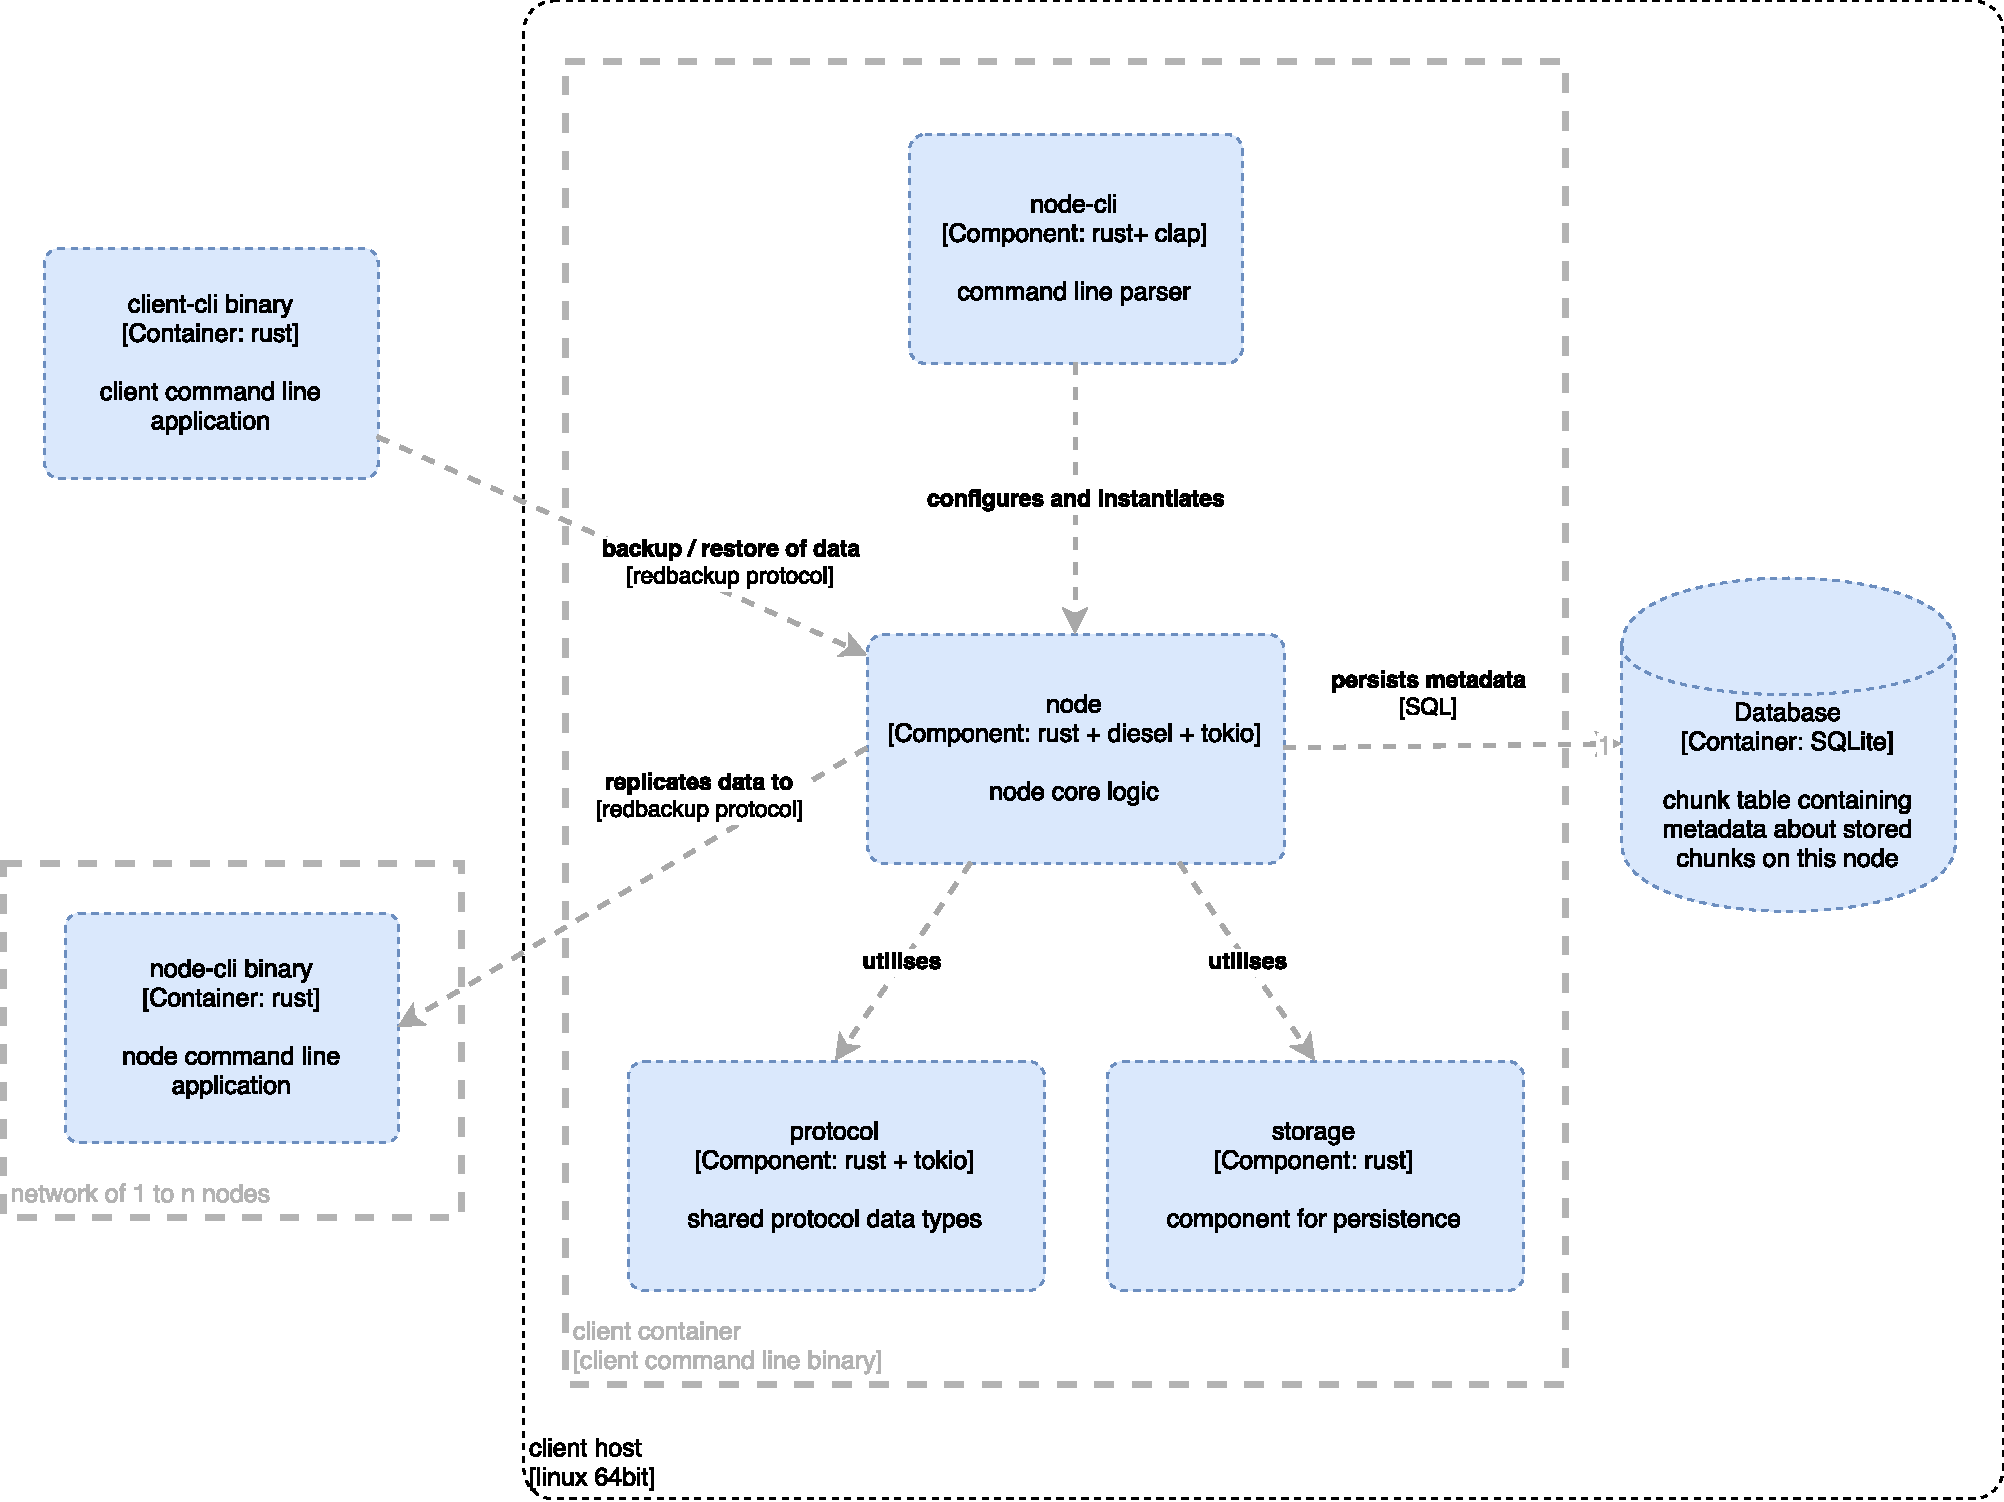
\includegraphics[width=1\linewidth]{resources/c4-node-container}
	\caption[Node specific C4 Container diagram]{C4 Container diagram illustrating the shape of the \gls{node} and how responsibilities are distributed as implemented in the study project.}
	\label{fig:c4-node-container}
\end{figure}

Exactly like the \gls{client} implementation, the command line logic is encapsulated in a separate component called \emph{node-cli}.

The core logic is implemented in the \emph{node} library. Like the client, the \gls{node} component makes heavy use of the tokio and Diesel library. In contrast to the client, we used the parallel features of tokio. To keep the chosen technology close to the client, we decided to use SQLite to store metadata about the data \glspl{chunk} present on the \gls{node} as well. This must be changed in the future because SQLite locks the entire database when writing, which makes concurrent updates impossible \cite{sqlite-locking}.

We use the same \emph{protocol} component for (de-) serialisation of messages on the \gls{node} and the \gls{client}.

The \emph{storage} component is also bundled directly in the \gls{node} executable. It persists data in one single directory as described in \fullref{sec:fundamental-design-decisions}.

Other known \glspl{node} are passed to the \gls{node} executable via command line arguments.

Because user authentication is complex and requires additional cryptographic efforts, the prototype accepts backups and replications from everyone.

\subsection{Testing}\label{testing}

In the following subsections, we describe how we tested our prototype and architecture.

\subsubsection{Unit Tests}\label{unit-tests}
We used test driven development (TDD) to develop the prototype as much as possible. Our Definition of Done\cite{project-plan} states that \emph{reasonable unit and integration tests [must] exist and pass.}

All unit tests were executed on every build run of our continuous integration. That is on every repository push and pull request.

Some unit tests written for the prototype are not pure unit tests but minimal integration tests. Because Rust is not a traditional object-oriented language, it is not possible to introduce and use interfaces (Traits) in the same way as we were used to from other languages such as Java or C\#. Due to the steep learning curve Rust has, we were not able to fully utilise the corresponding mechanisms.

\subsubsection{Integration Tests}\label{integration-tests}

Our integration tests are split into two main environments: A minimal one as defined in Figure \ref{fig:integrationtestsmall} and a medium network, as defined in Figure \ref{fig:integrationtestmedium}.

\begin{figure}
	\centering
	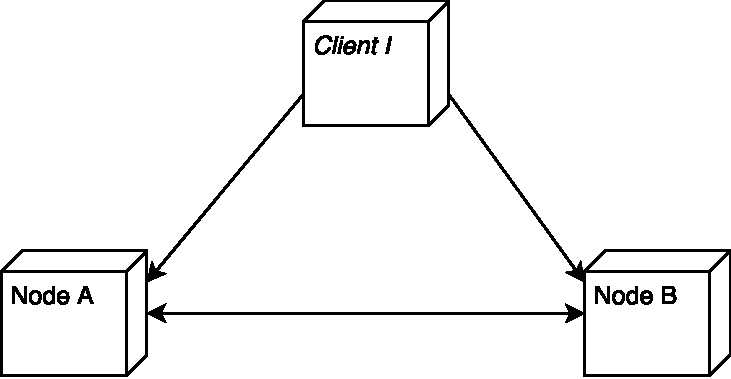
\includegraphics[width=0.5\linewidth]{resources/integration_test_small}
	\caption[Minimal integration test]{Minimal integration test with one \gls{client} and two \glspl{node}.}
	\label{fig:integrationtestsmall}
\end{figure}

\begin{figure}
	\centering
	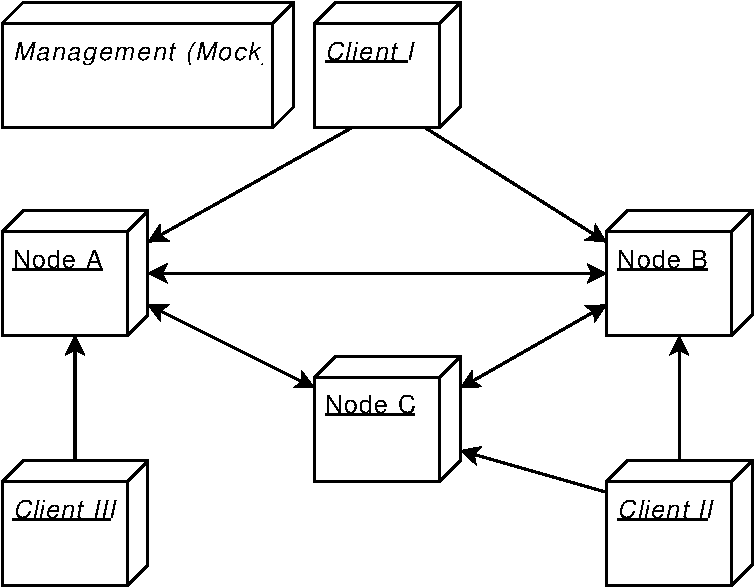
\includegraphics[width=0.5\linewidth]{resources/integration_test_medium}
	\caption[Medium integration test]{Medium integration test with three \glspl{client} and three \glspl{node}.}
	\label{fig:integrationtestmedium}
\end{figure}

These two rather small network styles will probably be the most commonly used deployments, yet cover most of the possible problems that may occur.

The integration tests are run automatically at least on every tagged release (i.e. at least once every sprint). Because of the (yet) small set of integration tests we wrote for the prototype, we ran the tests on every build.

To write comprehensive black box integration tests, we created a testing library written in Python\footnote{\url{https://www.python.org/}}. In this framework, the internals on how to launch and configure \glspl{client} and \glspl{node} is encapsulated in classes. Using this abstraction, we decided to launch \glspl{client} and \glspl{node} in separate Docker\footnote{\url{https://www.docker.com/}} containers, so that they are as isolated as possible. All containers used in a test case are connected to a dedicated Docker network, which eliminates possible interferences with other network services.

We wrote integration tests that verify that a backup are flawlessly created, restored and replicated onto other \glspl{node}.

Tests for fault tolerance, e.g. what happens if a \gls{node} goes down during a backup, can be implemented as integration tests as well.

\subsubsection{Test coverage}

Because Rust is still a young language with a relatively small ecosystem, tools for measuring code quality are still rare and immature. For our unit tests, we used Tarpaulin\footnote{\url{https://github.com/xd009642/tarpaulin}} to generate code coverage. Tarpaulin does not (yet) cover all language features and therefore returns a conservative coverage number. We achieved 53.5\% line coverage taking into account that this number would be significantly higher if all executed lines were counted (e.g. generated code using macros as well as compiler optimisations are not counted).
Code coverage achieved using the integration tests is not yet supported by any tool known to us and therefore undocumented. The integration tests do however cover all positive scenarios that were implemented.

\subsubsection{Architecture tests}

Architectural tests are special and manually run tests to verify the scalability of our software architecture.

Our integration testing framework allowed us to write such tests in a simple fashion.

\paragraph{Size Scalability}
As per our requirements in Appendix \ref{requirements}, the architecture should scale up to 100 \glspl{node}.

To test this scenario, we used the same underlying techniques as in our integration tests (see chapter \ref{integration-tests}), but scale the infrastructure up to the required limits.

Due to the high memory consumption of our prototype, we were not able to conduct this test with a significant amount of data. We conducted one test, where a file of 5MB was replicated to 99 Nodes which did not show any loss in performance.

\paragraph{Data Capacity}
Our requirements (Appendix \ref{requirements}) also state, that a \gls{node} must be able to handle up to e.g. 2TB of data. To test this requirement, we planned to create large amounts of random data that has to be stored. This is a realistic requirement, as e.g. a compressed image, audio and movie collection might reach such sizes in practice.

Both, the \gls{client} and the \gls{node} of the prototype, use a lot of memory during the creation of a backup. It was therefore not possible yet to create a single backup of 2TB. Performing multiple backups in a row of a smaller dataset (i.e. 5 files with a size of 500MB) has not shown a decrease in performance.

\paragraph{Concurrent Backups}

We ran a test in which 5 \glspl{client} back up randomly generated data onto three randomly chosen \glspl{node}. On average, the complete backup process of 1MB data \gls{chunk} took 90-130ms from one docker container into another. In reality, where \glspl{client} and \glspl{node} are on separate physical machines,  this time will be higher due to network latency.

These tests are however are partly problematic because the creation of backups require a lot of CPU time for the calculation of hashes. Running all \glspl{client} on separate machines would probably improve the performance slightly.
